\section{Introduction}
The advancement of Intelligent Transportation Systems (ITS) has increased the importance and applicability of traffic prediction. Traffic prediction plays a pivotal role in enhancing road traffic efficiency and driver experience, supporting applications such as travel time estimation, congestion management, route guidance, and signal control for effective traffic flow management \cite{vlahogianni_short-term_2014}.
% Also, developments in Internet of Things (IoT) technologies have grown the volume and variety of data collected within the transportation domain. 
The availability of extensive traffic data, particularly from network-wide loop detectors, has enhanced the development and validation of traffic prediction models.
For example, the Performance Measurement System (PEMS) provides link-level traffic data such as flow, speed, and density (occupancy)  at 5-minute intervals from thousands of loop detectors deployed across road networks \cite{chen_freeway_2001}, covering freeways across major metropolitan areas of California, USA, as shown in Figure~\ref{fig:sensor_maps}.

\begin{figure}[htbp]
  \centering
  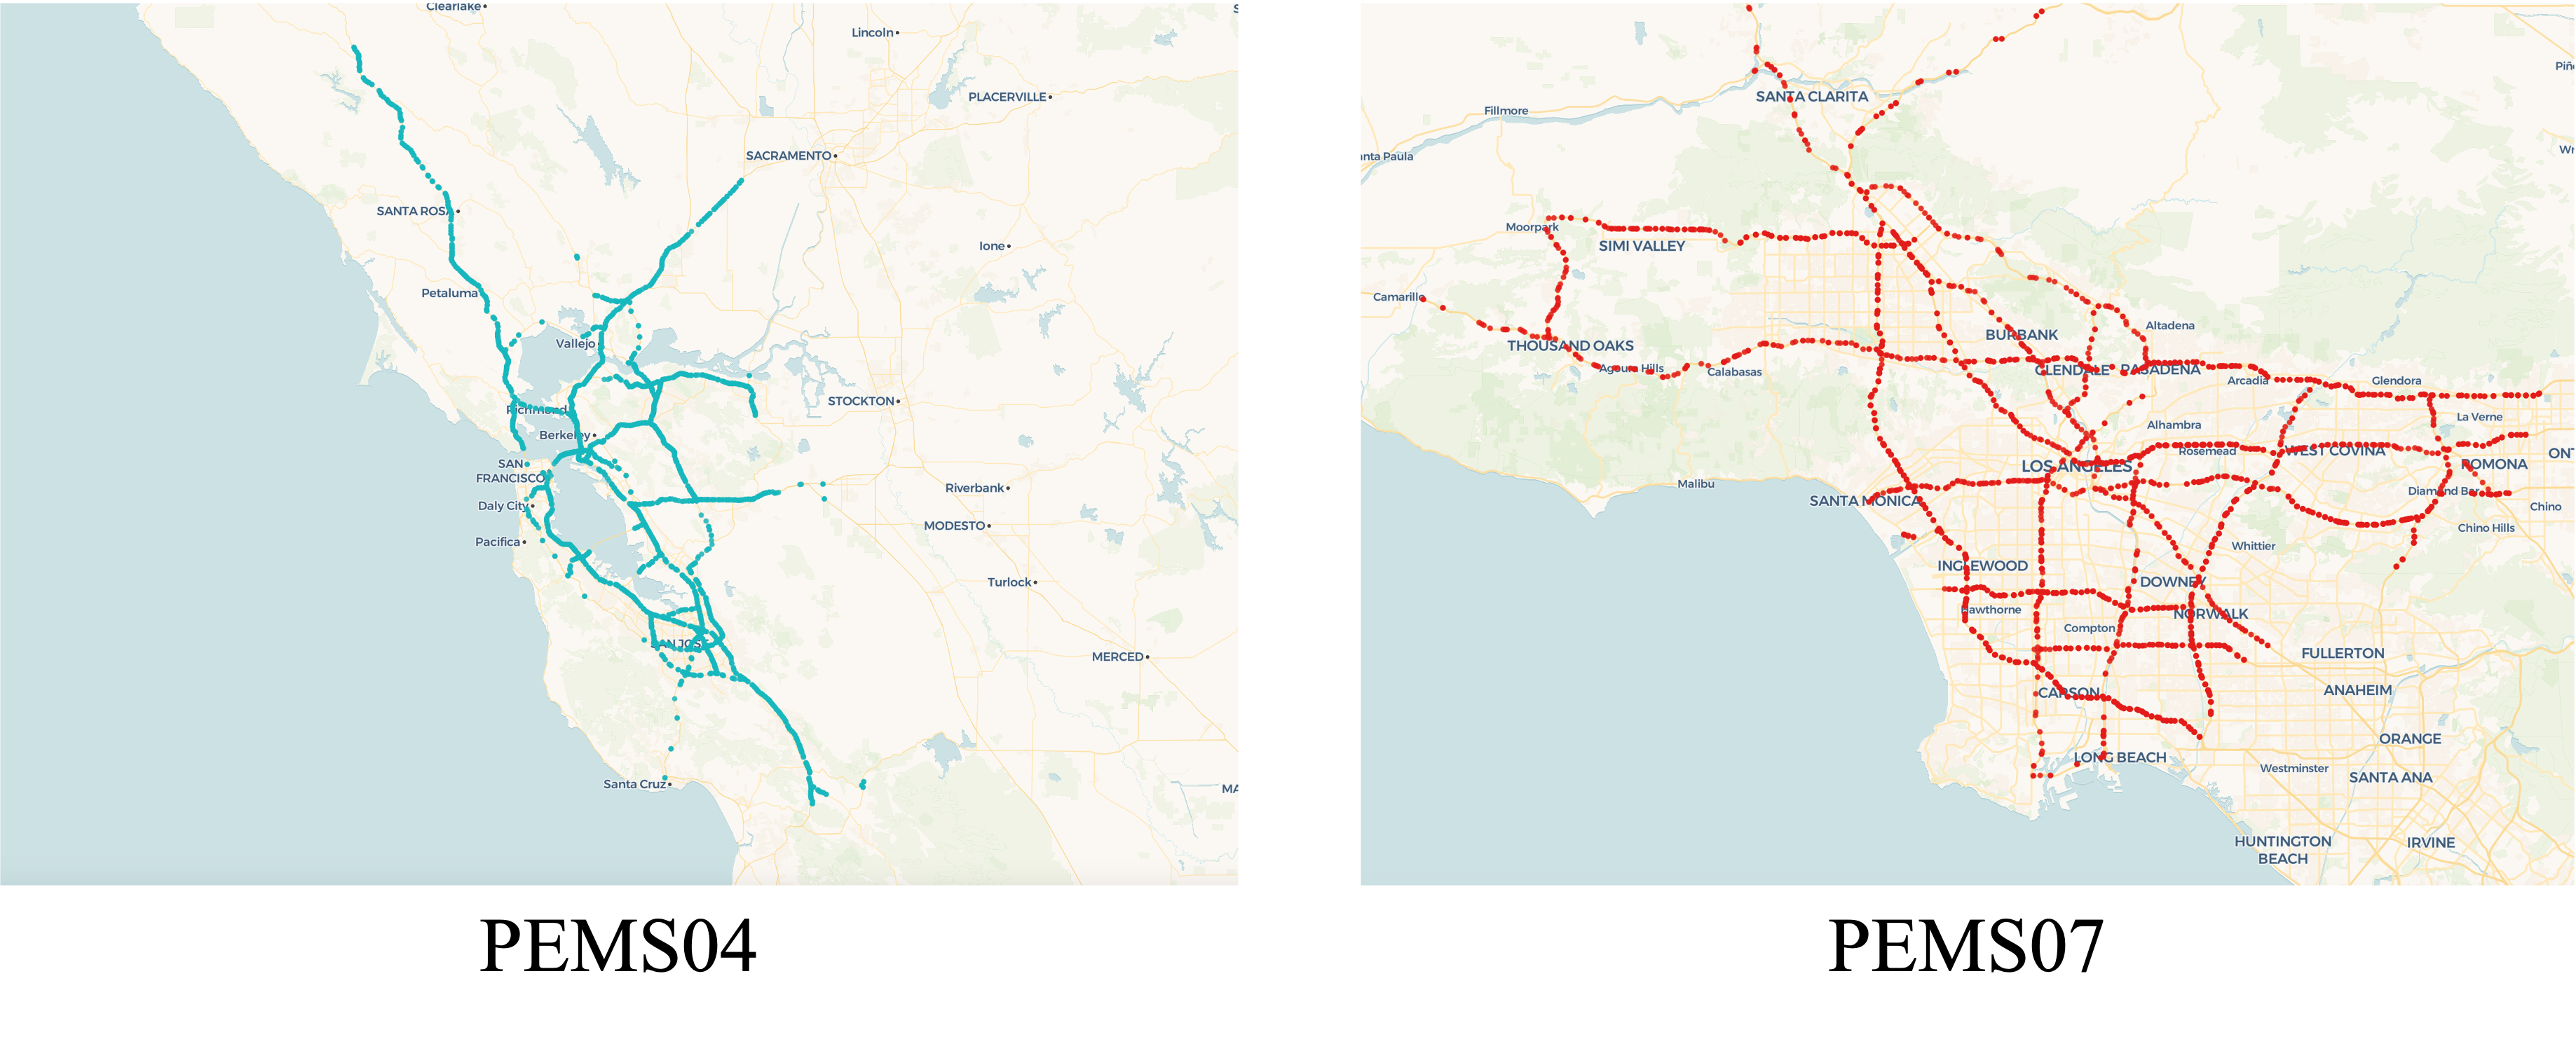
\includegraphics[width=0.9\linewidth]{figures/sensor_map.png} 
  \caption{Geographical distribution of traffic sensors in the PEMS04 (left, Bay Area) and PEMS07 (right, Los Angeles) datasets evaluated in this study.}
  \label{fig:sensor_maps}
\end{figure}

Recent innovations in machine learning have investigated application of Graph Neural Networks (GNNs) for traffic prediction \cite{yin_deep_2021}. These models capture the complex spatio-temporal dependencies in traffic data and have demonstrated superior performance compared to traditional time-series forecasting methods such as Autoregressive Integrated Moving Average (ARIMA) and other machine learning models for sequential prediction such as Long Short-Term Memory (LSTM)~\cite{wu_graph_2019, cui_traffic_2019}. However, GNN models require substantial training data and extensive computation, causing challenges related to training time and resources.
Recent benchmark study shows several state-of-the-art GNNs suffer from long training time due to their increased model complexity\cite{liu_largest_2023}.
% either require more than 100 GPU-hours or cannot be trained at all within practical resource limits \cite{liu_largest_2023}.

In computer vision research area, various techniques have been proposed to lower the computational burden associated with training complex models on large datasets. \textit{Coreset} selection, the task of identifying a small, representative subset of data samples from original dataset, has demonstrated significant advances in image classification tasks. Applied to benchmarks like CIFAR-10, CIFAR-100, and ImageNet-1k, it has demonstrated the potential to significantly reduce training resources with minimal impact on model performance. Recent studies \cite{xia_moderate_2022, maharana_d2_2023, tan_data_2025} indicate that models trained on coresets using only 50\% of the original data can achieve predictive performance with only a small degradation (e.g., less than a 5\% drop). Minimising the dataset size with small performance loss offers decreased training time and computational cost. This accelerates model development and deployment cycle, by enabling faster experimentation and optimisation.

In contrast, applying coreset selection to multivariate time-series forecasting such as traffic prediction has received limited attention. Multivariate time-series data commonly contain strong periodicities (e.g., daily, weekly cycles), creating data redundancy. At the same time, these datasets frequently include unique but potentially important events or anomalies. Therefore, the selection of coreset in this domain must balance reducing data redundancy and keeping essential pattern information.
Thus, systematically investigating coreset selection for large-scale multivariate time-series forecasting can improve computational efficiency and forecasting accuracy, opening diverse application opportunities.

In this paper, we present a comprehensive investigation into the application of coreset selection methods for traffic prediction. We evaluated eight coreset selection methods. We apply these methods to the traffic prediction task based on a GNN model using two benchmark datasets. Our findings shed light on both the potential benefits and limitations of employing coreset selection in traffic forecasting. 

\begin{figure*}[t] 
  \centering
  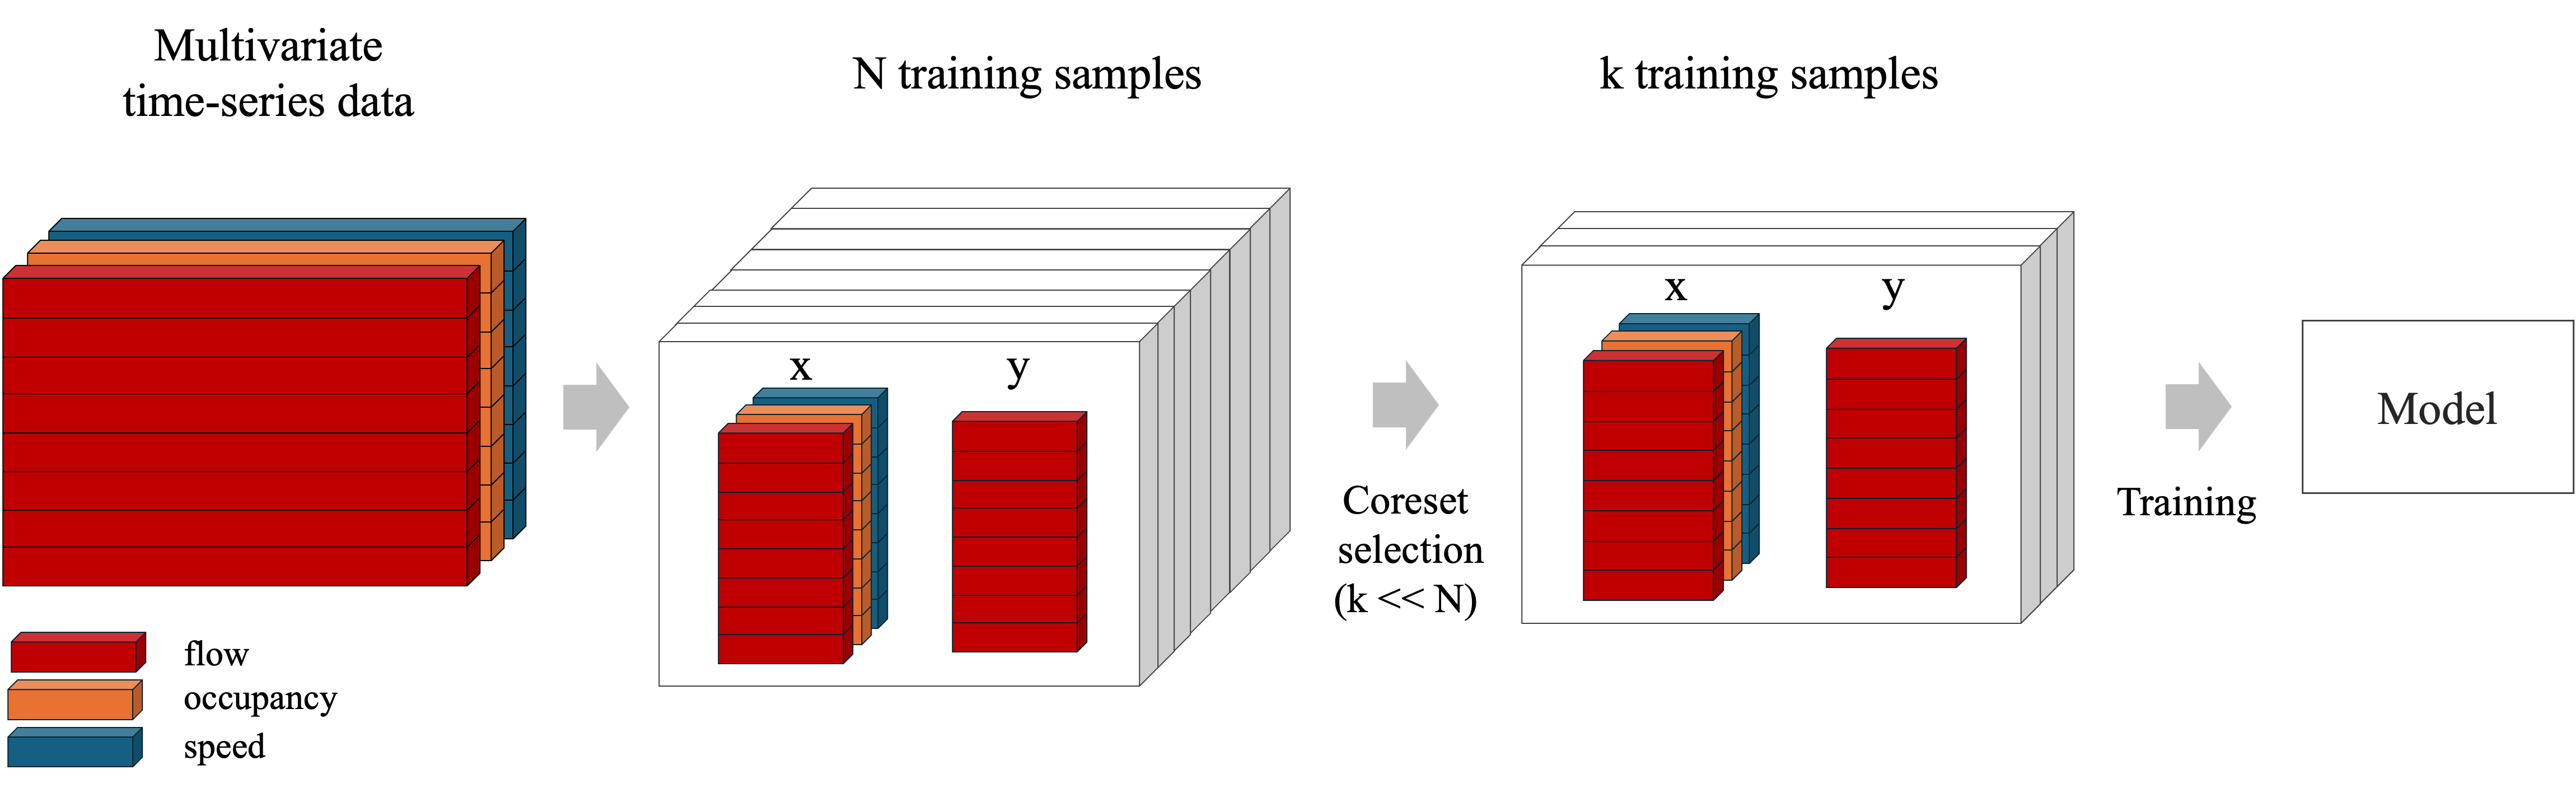
\includegraphics[width=\linewidth]{figures/overall.png} 
  \caption{Overall pipeline of applying coreset selection for traffic forecasting model training.}
  \label{fig:overall_workflow}
\end{figure*}
% ----------------------------------

The main contributions of this paper can be summarised as follows:
\begin{itemize}
    \item To the best of our knowledge, we present the first systematic benchmark evaluating eight model-free coreset selection methods for large-scale GNN-based traffic forecasting. 
    \item We demonstrate that model performance using a coreset depends on achieving good feature‐space coverage. Furthermore, we show that for spatio-temporal traffic data, preserving temporal diversity is an effective strategy to help attain this crucial feature coverage.

    \item We empirically validate that using only 30-50\% coresets maintains prediction accuracy near the accuracy of full-data baseline. We also observe that certain coresets (often 50-90\% ratio) slightly outperformed models trained on the entire dataset.
\end{itemize}